
\chapter{Flavour Tagging with Graph Networks and Transformers}
\label{ch:spice}

In this chapter we describe the design and implementation new graph networks for flavour tagging.
Jet flavour tagging is a crucial part of the ATLAS experiment and is described in \Cref{sec:flavour_tagging}.
These models attempt to identify the flavour of a jet based on the properties of the reconstructed charged particle tracks associated with it.

The new models build on GN1, a graph network which uses GATv2 system of message passing~\cite{GATv2}.
The first new model is called GN++ and is based on the full GN Block architecture described in \Cref{sec:gn_block}, complete with persistent edge information and global attributes.
The second new model is called Spice and is based on the transformer-encoder architecture, described in \Cref{sec:transformer}.
Spice would prove to be so performant and efficient that it would form the basis of the new GN2 flavour tagger adopted by the ATLAS collaboration.

One of the observations made over the course of this project is that the rate of progress in machine learning is much faster than in high energy physics.
At the time Spice was being developed and presented to the flavour tagging group, GN1 was still undergoing collaboration.
At the time of writing, GN2 is now being calibrated, and significant effort is being used to keep it up to date with the latest developments in machine learning.
One of the main contributions of this thesis was the development of Salt~\cite{Salt}, a repository for training transformers for flavour tagging which is constantly being updated with the latest models and training techniques.

\section{Datasets}

Training and evaluating GN++ and Spice required the use of simulated datasets in order to provide a ground truth for the jet flavour.
This work reuses the same samples as the previous flavour taggers, DIPS and GN1, and further information can be found in \textcite{AlexThesis} and Ref.~\cite{GN1}.
The training datasets are selected to cover a wide range of $\pt$ values and further resampled to ensure that the jet $\pt$ and $\eta$ distributions are identical for the three jet flavours used in the classification, namely $b$-, $c$-, and light-jets.

Two simulated datasets are used.
The first dataset comprises $\ttbar$ events, primarily covering the $\pt < 250~\GeV$ phase space.
The simulation settings for this sample were derived from best fits of the data distributions for jet multiplicity and top quark momentum~\cite{ttbar1, ttbar2}.
The second dataset consists of $Z'$ events, included to enhance the training statistics in the high $\pt$ phase space.
The $Z'$ boson, a non-SM particle, is designed explicitly with cross-section of the hard scattering process adjusted to produce a flat mass distribution, leading to a relatively uniform distribution of jets with $\pt$ up to $5~\TeV$.
The branching fractions were also tuned to result in a roughly equal distribution of $b$-, $c$-, and light-jets at $\pt \approx 3~\TeV$.
The branching fractions of the $Z'$ boson shown in \Cref{tab:zprime_branching}.

Distributions of the jet $\pt$ and $\eta$ for the two datasets are shown in \Cref{fig:jet_pt_eta}.

\begin{table}[h]
    \centering
    \begin{tabular}{lcc}
        \toprule
        \midrule
        Decay Mode & Branching Fraction \\
        \midrule
        $b\bar{b}$ & 0.30 \\
        $c\bar{c}$ & 0.30 \\
        $s\bar{s}$ & 0.10 \\
        $d\bar{d}$ & 0.10 \\
        $u\bar{u}$ & 0.10 \\
        $\tau^-\tau^+$ & 0.05 \\
        $e^-e^+$ & 0.05 \\
        \bottomrule
    \end{tabular}
    \caption{Branching fractions for the $Z'$ boson \cite{Run2FTAlgs}}
    \label{tab:zprime_branching}
\end{table}


\begin{figure}
    \centering
    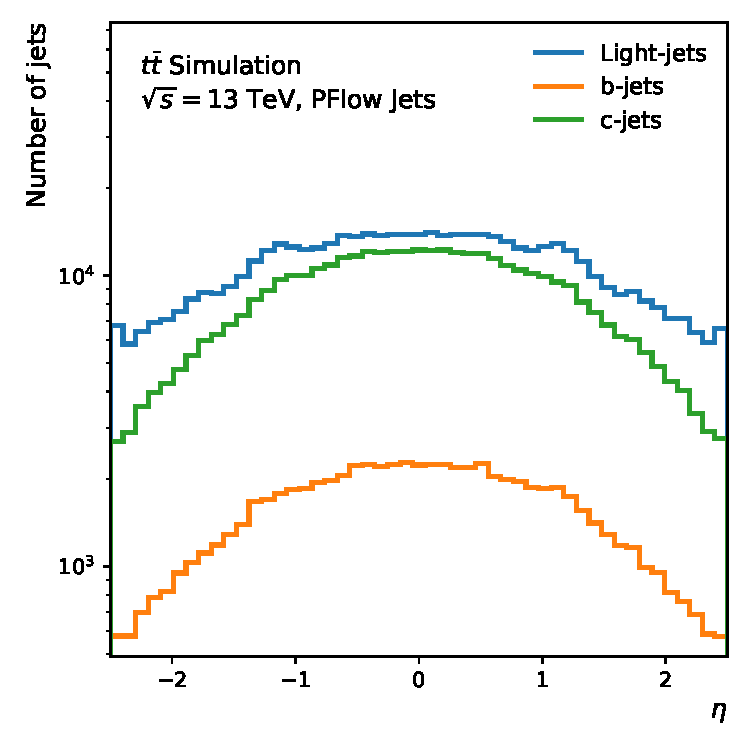
\includegraphics[width=0.45\textwidth]{figures/flavour_tagging/ttbar_0.pdf}
    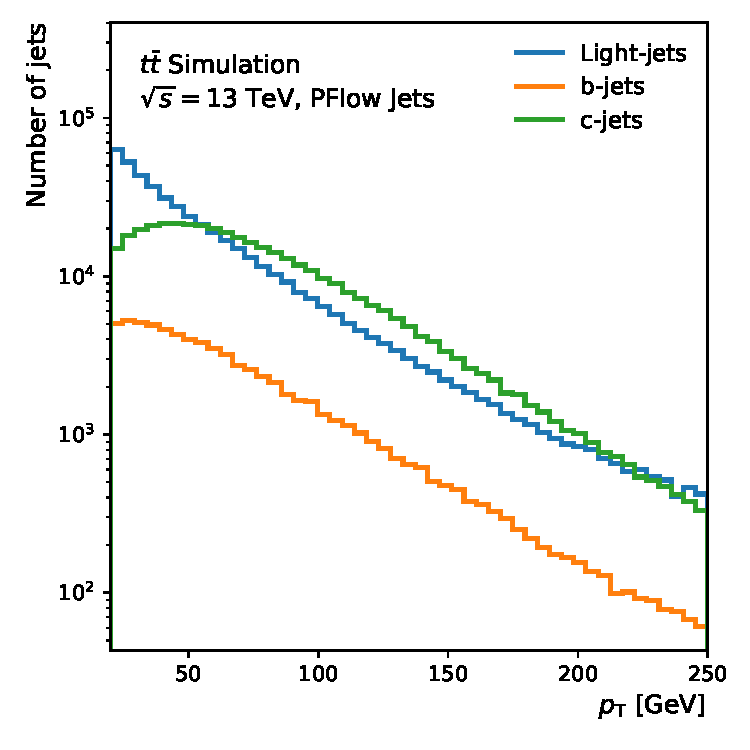
\includegraphics[width=0.45\textwidth]{figures/flavour_tagging/ttbar_1.pdf}
    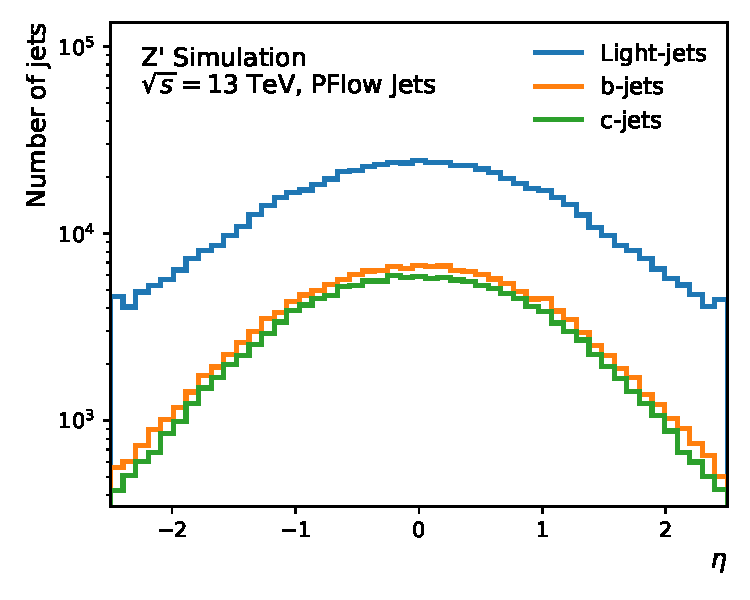
\includegraphics[width=0.45\textwidth]{figures/flavour_tagging/zprime_0.pdf}
    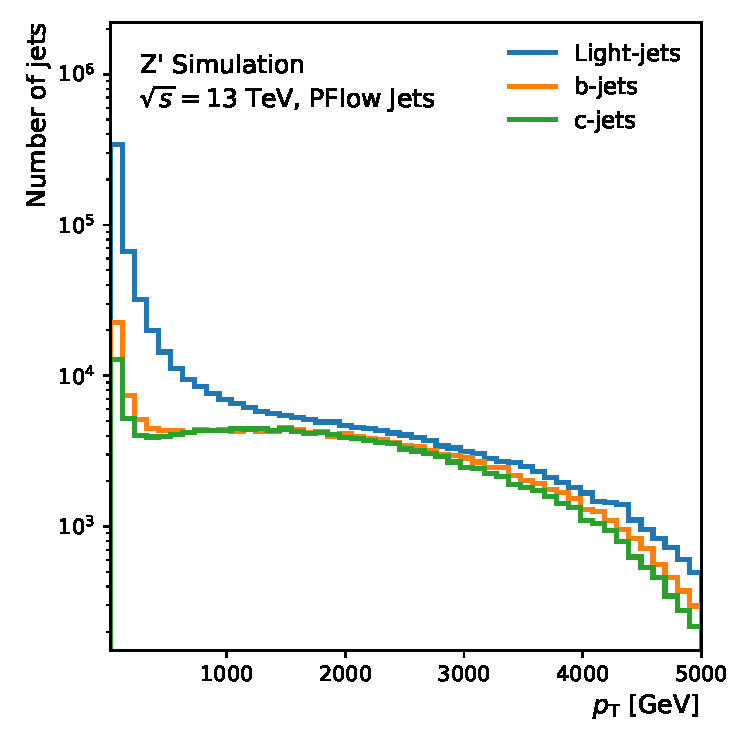
\includegraphics[width=0.45\textwidth]{figures/flavour_tagging/zprime_1.pdf}
    \caption{Original non-resampled jet $\pt$ (left) and $\eta$ (right) distributions for the $\ttbar$ (top) and $Z'$ (bottom) datasets.}
    \label{fig:jet_pt_eta}
\end{figure}

\subsection{Monte Carlo Generation}

Both datasets are initiated by simulated proton-proton collisions at a center-of-mass energy of $\sqrt{s} = 13$ TeV.

Hard scatter events for the $\ttbar$ sample were generated at next-to-leading order using \textsc{PowhegBox v2}~\cite{Powheg1, Powheg2, Powheg3}.
These events then interfaced with \textsc{Pythia 8.230}~\cite{Pythia8} using the \textsc{A14} tune~\cite{A14} for parton showering and hadronization.
For the parton distribution functions, the \textsc{NNPDF3.0NNLO}~\cite{PDF3.0} set was used for the matrix element calculation while the \textsc{NNPDF2.3LO}~\cite{PDF2.3} set was used for the showering.
The cut-off scale parameter for the first-gluon-emission $h_{\text{damp}}$ was set to 1.5 times the top quark mass of $m_t = 172.5~\GeV$.
The $Z'$ sample was generated and showered using \textsc{Pythia 8.212} with the \textsc{A14} tune and the \textsc{NNPDF2.3LO} set of parton distribution functions.
The flat mass distribution of the $Z'$ boson was achieved by applying a per-event weight to broaden the natural decay width of the $Z'$ boson.

For both datasets, decays of $b$- and $c$-hadrons were simulated using the \textsc{EvtGen v1.6.0} package \cite{EvtGen}.
Detector response was performed using the \textsc{Geant4} simulation package~\cite{Geant4} with the ATLAS simulation setup~\cite{ATLASSim}.
These signals are combined with the hard scatter events during the digitization step.
Interactions with heavy flavour hadrons and the detector material was not simulated but accounted for in correction factors and systematic uncertainties.
Pileup was modelled by overlaying extra minimum bias events using the \textsc{Pythia 8.160} generator with the \textsc{A3} tune~\cite{A3} and the \textsc{NNPDF2.3LO} parton distribution functions.
In-time pileup was modelled using an average of 40 interactions per bunch crossing, while out-of-time pileup was modelled using bunch crossings before and after the primary interaction.

\subsection{Reconstruction}

The output of the simulation was reconstructed using the standard ATLAS reconstruction procedure described in \Cref{sec:event_reconstruction}.
In these experiments, the inputs to the model stem from the tracks and no calibrated physics objects, such as reconstructed photon, electrons, or muons, are used.

Charged particle tracks are required to pass the loose selection criteria~\cite{TrackLoose} as shown in \Cref{tab:track_loose}.
The hard scatter primary vertex (PV) is defined as the vertex with the highest sum of squared transverse momenta of the associated tracks.
The impact parameters (IPs) for each track are measured with respect to the PV of the event.
Jets are reconstructed from particle-flow objects~\cite{PFlow} using the anti-$k_t$ algorithm with a radius parameter of $R = 0.4$.
More details are covered in \Cref{sec:particle_flow}.
Tracks are associated to a jet based on the $\Delta R$ separation to the jet axis.
The threshold decreases as a function of the jet $\pt$ to account for the increased collimation of the jet cone, from $\Delta R = 0.45$ at $\pt = 20~\GeV$ to $\Delta R = 0.25$ at $\pt \geq 200~\GeV$.
If a track associated with multiple jets, it is assigned to the jet with the smallest $\Delta R$ separation.

\begin{table}
    \centering
    \begin{tabular}{ll}
        \toprule
        $\pt$ & $> 1~\GeV$ \\
        $d_0$ & $< 3.5~\mm$ \\
        $z_0 \sin \theta$ & $< 5~\mm$ \\
        Number of hits in the SCT & $\geq 8$ \\
        Number of hits shared by other tracks & $\leq 2$ \\
        Number of SCT holes & $\leq 3$ \\
        Number of pixel holes & $\leq 2$ \\
        \bottomrule
    \end{tabular}
    \caption{Loose selection criteria for charged particle tracks~\cite{TrackLoose}.}
    \label{tab:track_loose}
\end{table}

\subsection{Truth Labelling}

As with GN1, these networks are trained to perform three complimentary tasks.
There is task is the classification of the jet flavour, this is the primary task.
The second task is to predict the origin of each track within the jet.
The final task is to segment the jet: given any two tracks from the same jet, determine if they emerged from the same vertex.
Each of these requires defining ground truth labels.

The truth labelling of the jets is based on the existence of generator level particles within a $\Delta R$ separation of 0.3.
The jet is associated with the particle with the highest priority within this radius.
The considered particles in order of decreasing priority are, $b$-hadrons, $c$-hadrons, and $\tau$ leptons, which will result in the jet being labelled as a $b$-jet, $c$-jet, $\tau$-jet respectively.
If no such particles are found, the jet is labelled as a light-jet.
We discard $\tau$-jets for this study.

The truth track origins describe the physical process which produced the track.
First a track is associated with a truth particle by matching its reconstructed hits to the simulated hits of the particle made during the \textsc{Geant4} simulation.
This matching criteria is performed using the~\textit{truth-matching probability} (TMP)~\cite{TMP}.
The TMP constructs a ratio of the matched hits to the total number of hits in the track, with added factors to account for the varying hit efficiencies of the detector subcomponents, namely the pixel, SCT, and TRT detectors.
Each track is associated to the truth particle with the highest TMP.
If no truth particle leads to a TMP greater than 0.75, the track is labelled as a fake track, and it is determined to have originated from multiple overlapping particles.
There are eight possible truth labels for the tracks as shown in \Cref{tab:track_labels}.

\begin{table}
    \centering
    \begin{tabular}{ll}
        \toprule
        $b$-hadron decay \\
        $c$-hadron decay which itself originated from a $b$-hadron \\
        other $c$-hadron decay \\
        $\tau$-lepton decay \\
        other secondary decays (such as kaons) \\
        the primary vertex \\
        a pileup $pp$ interaction \\
        a fake track from multiple overlapping particles \\
        \bottomrule
    \end{tabular}
    \caption{The eight possible truth labels for the tracks.}
    \label{tab:track_labels}
\end{table}

Finally, the truth vertex labelling is based on the origin of the tracks.
This is a simple binary label which determines if a pair of tracks emerged from the same secondary vertex within the jet.
The label is set to True if the associated truth particles of each track share an origin within $1~\mm$ of each other.
If one of the tracks is labelled as ``Fake'' or ``Pileup'', the pair is always labelled as False.

\subsection{Selection and Sampling}

Jets are required to have $\pt > 20~\GeV$ and $|\eta| < 2.5$ and may not overlap with a generator-level lepton from a $W$ or $Z$ decay.
From the $Z'$ sample, jets are further required to have $\pt > 250~\GeV$ to avoid simulation artefacts.
All jets with $\pt < 60~\GeV$ and $|\eta| < 2.4$ must also pass the tight working point of the JVT algorithm in order to minimize contributions from pileup~\cite{JVT}.

As shown in \Cref{fig:jet_pt_eta}, there is a significant difference between the jet $\pt$ and $\eta$ for the three jet flavours.
This would bias the training of the model and lead to issues down the line for calibration.
To mitigate this, the training dataset is resampled with replacement to ensure that the 2D distribution of jet $\pt$ and $\eta$ is identical for the three jet flavours~\cite{AlexThesis}.

After resampling the training set contained a total of 120 million jets split equally between the three jet flavours and composed of a mixture of around 70\% $\ttbar$ and 30\% $Z'$ events.
The distributions of the jet $\pt$ and $\eta$ for the resampled datasets are shown in \Cref{fig:train_jet_pt_eta}.
During training, 5\% of this was reserved for hold out validation.

Two statistically independent test samples were produced, each containing 1 million $\ttbar$ and $Z'$ jets respectively.
No resampling was performed on the test datasets.

\begin{figure}
    \centering
    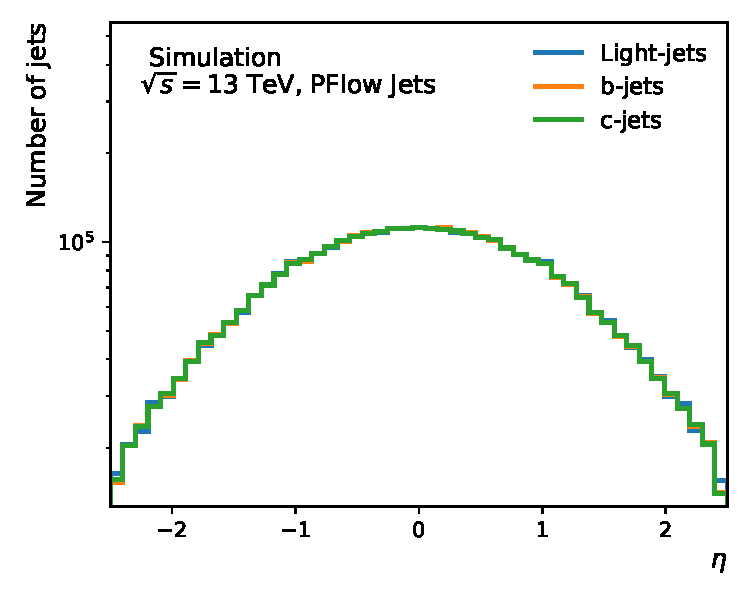
\includegraphics[width=0.45\textwidth]{figures/flavour_tagging/train_0.pdf}
    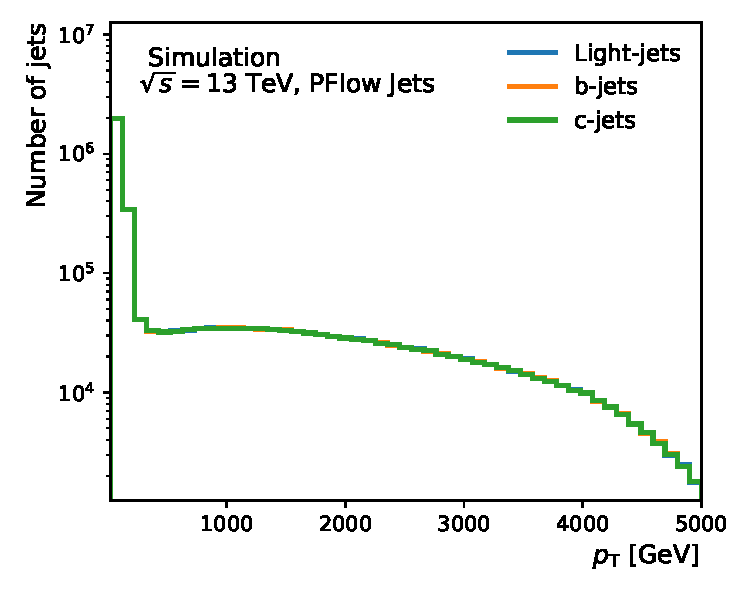
\includegraphics[width=0.45\textwidth]{figures/flavour_tagging/train_1.pdf}
    \caption{Resampled jet $\pt$ (left) and $\eta$ (right) distributions for the training dataset. For these plots only 10M jets were selected as a representative sample.}
    \label{fig:train_jet_pt_eta}
\end{figure}

\subsection{Input Features}

The inputs to all models are the same as those used in GN1.
They include two kinematic jet variables, $\pt$ and $\eta$, and up to 40 tracks associated with the jet.
Each track is represented by a vector containing 21 features, detailed in \Cref{tab:track_features}.
Almost all $\ttbar$ jets contain less than 40 tracks, but a significant fraction of $Z'$ jets contain more, as shown in \Cref{fig:track_multiplicity}.
For these samples only the 40 tracks with the highest transverse IP significance $s(d_0)$ are retained.
All features are standardized to have zero mean and unit variance using the training set statistics.

\begin{figure}
    \centering
    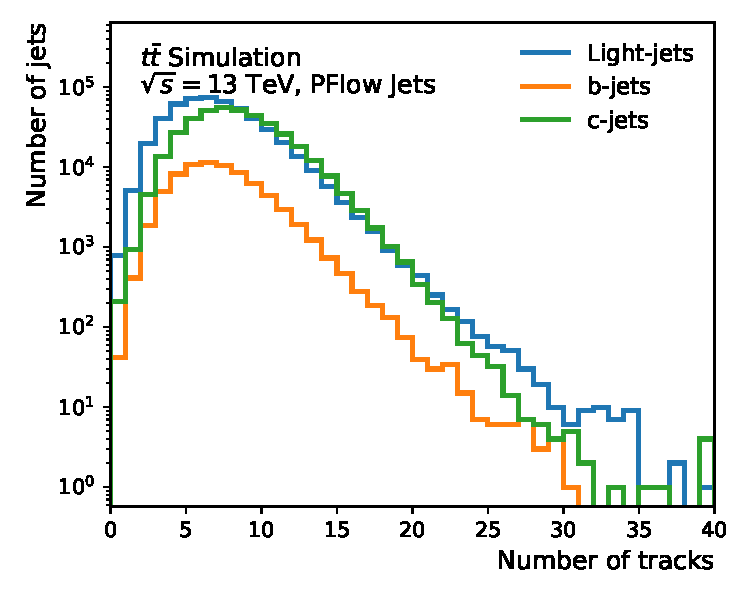
\includegraphics[width=0.45\textwidth]{figures/flavour_tagging/ttbar_2.pdf}
    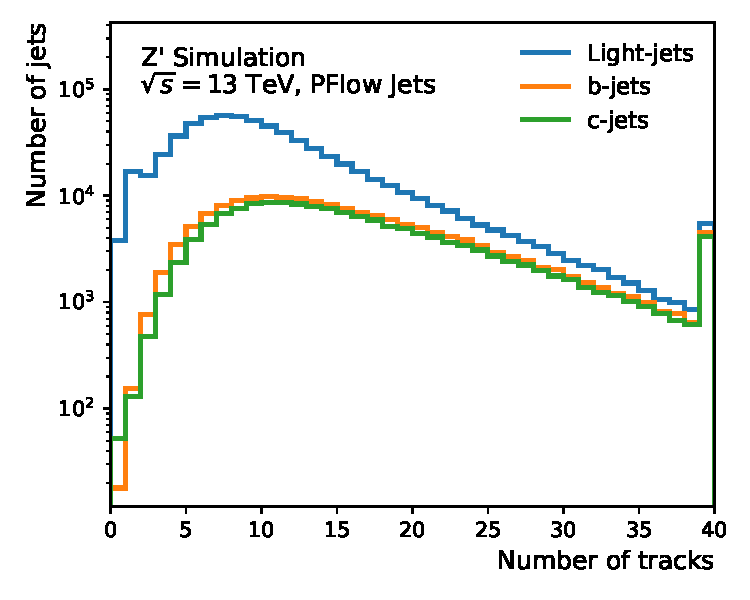
\includegraphics[width=0.45\textwidth]{figures/flavour_tagging/zprime_2.pdf}
    \caption{Original non-resampled number of tracks associated with each jet in the $\ttbar$ (left) and $Z'$ (right) datasets.}
    \label{fig:track_multiplicity}
\end{figure}

\begin{table}[h]
    \centering
    \begin{tabular}{ll}
        \toprule
        \midrule
        \multicolumn{2}{c}{Jet level inputs} \\
        \midrule
        $\pt$ & Jet transverse momentum \\
        $\eta$ & Signed jet pseudorapidity \\
        \midrule
        \midrule
        \multicolumn{2}{c}{Track level inputs} \\
        \midrule
        $q/p$ & Track charge divided by momentum \\
        $\Delta\eta$ & Pseudorapidity of the track relative to the jet $\eta$ \\
        $\Delta\phi$ & Azimuthal angle of the track relative to the jet $\phi$ \\
        $d_0$ & Closest distance from the track to the PV in the longitudinal plane \\
        $z_0 \sin \theta$ & Closest distance from the track to the PV in the transverse plane \\
        $\sigma(q/p)$ & Uncertainty on q/p \\
        $\sigma(\theta)$ & Uncertainty on track polar angle $\theta$ \\
        $\sigma(\phi)$ & Uncertainty on track azimuthal angle $\phi$ \\
        $s(d_0)$ & Lifetime signed transverse IP significance \\
        $s(z_0)$ & Lifetime signed longitudinal IP significance \\
        nPixHits & Number of pixel hits \\
        nSCTHits & Number of SCT hits \\
        nIBLHits & Number of IBL hits \\
        nBLHits & Number of B-layer hits \\
        nIBLShared & Number of shared IBL hits \\
        nIBLSplit & Number of split IBL hits \\
        nPixShared & Number of shared pixel hits \\
        nPixSplit & Number of split pixel hits \\
        nSCTShared & Number of shared SCT hits \\
        nPixHoles & Number of pixel holes \\
        nSCTHoles & Number of SCT holes \\
        \bottomrule
    \end{tabular}
    \caption{Input features for the graph network flavour taggers.}
    \label{tab:track_features}
\end{table}

\section{Model Design}

All the proposed models can be thought of as variations or extensions of GN1.
Both Spice and GN++ follow this same setup but with updates to the message passing steps as well as latest trends in architecture design.
From~\textcite{RelationalInductiveBiases} comes the design of the GN Block which include features such as, persistent edge information, persistent global information, and node feed-forward layers.
In addition, we experimented with the transformer architecture along with, PreNorm, conditioning, and residual additive connections which were back fitted to the GN Block.

GN1 introduced the idea of a monolithic graph neural network which would simultaneously perform jet tagging, track identification, and vertexing.
The input data is a set attributed nodes (the tracks) with an associate global attribute (the jet kinematics), with no explicit graph structure or edges features.
The three training objectives are equivalent to performing a graph level tasks, a node level task, and an edge level task respectively.
Thus, one can think of these models as mappings from the graph structure $(\mathcal{N}, \emptyset, \u) \rightarrow (\mathcal{N}', \mathcal{E}', \u')$, and the loss is calculated on each of the three outputs.

For all the models, while the edges are featureless, they are designed to be fully-connected, meaning that each node sends a message to every other node in the graph.
This was found to improve performance of all models, and the computational overhead was not significant, as the number of tracks per jet was limited to 40.
To compare these models we use flowcharts of the operations within the layers.
Theses flowcharts are shown in \Cref{fig:gn1_graph}, \Cref{fig:gnpp_graph}, \Cref{fig:gnmm_graph}, and \Cref{fig:spice_graph} and use the key shown in \Cref{fig:key}.

\begin{figure}
    \centering
    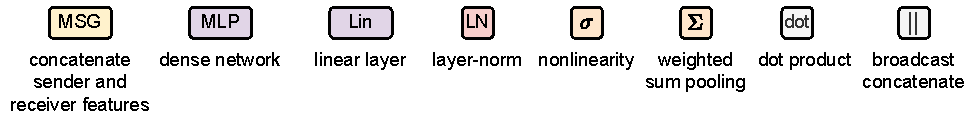
\includegraphics[width=0.99\textwidth]{figures/flavour_tagging/key.pdf}
    \caption{Key for the flowcharts of the graph network operations.}
    \label{fig:key}
\end{figure}

\subsection{GN1}

To better highlight the changes made in GN++ and Spice, we first describe the specifics of the GN1 model.
It is worth highlighting that we are comparing to the original GN1 implementation as described in Ref.~\cite{GN1}, as later variants began to adopt more transformer like features, such as multi-headed attention and multiple projection matrices before the full shift to Spice/GN2.

The model begins with a track initializer, which is an MLP that takes as inputs the concatenated track and jet features and outputs a track embedding of size 64.
The embedded track features are then passed through a three GATv2 layers~\cite{GATv2} to produce a set of updated track features.
In each layer the track features are projected using a learnable square matrix $\W$.
This is used to simultaneously calculate the message sent between each pair of tracks as well as the message weight using,
\begin{equation}
    e_{ij} = \text{softmax}_i\left(\ba \cdot \relu\left([\W \x_i, \W \x_j]\right)\right),
\end{equation}
where $\ba$ is a learnable vector, and $e_{ij}$ is the message weight sent from node $i$ to node $j$.
The softmax function is applied to all incoming messages to node $j$ to ensure that the weights sum to one.
The messages are then aggregated to update the node information across the graph,
\begin{equation}
    \x_j' = \relu\left(\sum_{i} e_{ij} \cdot \W \x_j\right).
\end{equation}
GN1 uses three of these layers to build its main feature extractor, returning a set of updated node features.
To perform the graph level task, the node features are aggregated using a weighted sum to create a pooled graph representation.
The weights of this sum are derived from another learnable projection on the final node features.
The pooled representation is passed through an MLP called the graph network to produce an output vector of size 3, which can be used for the classification task.
For the node task, the output of the last GATv2 layer is concatenated with the pooled graph representation and passed through another MLP called the node network with 8 outputs.
Finally, for the edge task, node features are concatenated in pairs, with both orderings, together with the pooled features and passed through a third MLP called the edge network 1 output.
In total GN1 has 820k trainable parameters and was implemented using the PyTorch Geometric library~\cite{PyTorchGeometric}.

A schematic diagram of the operations taking place within the GN1 graph network is shown in \Cref{fig:gn1_graph}.
Some notable limitations of the GN1 model are tied to the GATv2 layers.
The GATv2 layers reuse the same projection matrix $\W$ to calculate both the message content and the message weight.
These operations could be performed better with specialized layers.
Most notably missing is any strong nodewise updates after the message passing.
Framing this in the context of the GN Block means that the node update $\phi^x$ is simply a ReLU activation function.

\begin{figure}
    \centering
    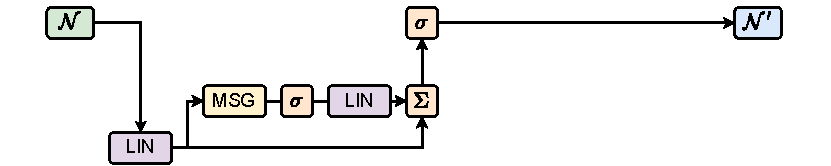
\includegraphics[width=0.99\textwidth]{figures/flavour_tagging/gn1.pdf}
    \caption{Diagram of the operations within one graph network layer of the GN1 tagger.}
    \label{fig:gn1_graph}
\end{figure}

\subsection{GN++}

The GN++ model is based on the full GN Block architecture described in \Cref{sec:gn_block}.
This model is designed to be a more expressive graph network than GN1, with persistent edge information and global attributes.
It also includes pre-normalization layers, residual connections, and multi-headed attention.
Other elements such as persistent global or edge information could also be added to the model.

\begin{figure}[h!]
    \centering
    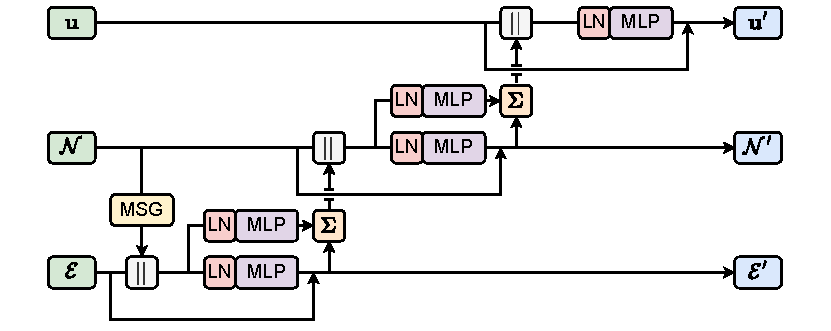
\includegraphics[width=0.99\textwidth]{figures/flavour_tagging/gnpp.pdf}
    \caption{Diagram of the operations within one graph network layer of the GN++ tagger.}
    \label{fig:gnpp_graph}
\end{figure}

A diagram of the information flow within the GN++ model is shown in \Cref{fig:gnpp_graph}.
In a single layer, there are 5 MLPs, 3 to perform the updates $\phi^x$, $\phi^e$, and $\phi^u$, and two to calculate the attention weights for the $\rho^{e \to x}$ and $\rho^{x \to u}$ steps.
The only part omitted from the GN Block is the $\rho^{e \to u}$ pooling operation as we found that it was computationally expensive and did not improve performance.
Each of the updates for the edges, nodes, and global attributes follows the same pattern, shown in the algorithm in \Cref{alg:gnpp} and by the diagram in \Cref{fig:gnpp_graph}.
Multi-headed attention is achieved by having multiple outputs for the $\rho^{e \to x}$ and $\rho^{x \to u}$ MLPs, and each are softmaxed separately.
All are additive residual and the weight matrix layer of the update MLPs are initialized with zeros.
All MLPs have a single hidden layer which doubles the embedding dimension, applies the LeaklyReLU activation, and projects back to the original.

For this model we keep the track initializer from GN1.
However, the three networks for the graph, node, and edge tasks are no longer required as the GN Block already has expressions for the node and edge tasks.
We simply change the output dimension of the final MLPs to match the required dimension of each task.
Edges and global information are empty for the first layer, after which they are initialized to have the same dimension as the node features.
For this residual connection, we pass the input through a linear resizing layer to match the output dimension.
We use 5 graph layers in total with half the embedding dimension of GN1 in order to have roughly the same number of parameters.
The GN++ model has 780k trainable parameters and was implemented using a custom build graph library in PyTorch.

The main differences between GN1 and GN++ are shown in \Cref{tab:gnpp_diff}.
For multi-headed attention we use four heads.
The minimal model, which we call GNA, is close to but not exactly the same as GN1.
A diagram of the operations taking place within the GNA graph network is shown in \Cref{fig:gna_graph}.

\begin{table}
    \centering
    \begin{tabular}{ll}
        \toprule
        \midrule
        Symbol & Description \\
        \midrule
        PE & Persistent edge information \\
        PG & Persistent global information \\
        NFF & Node feed-forward updates \\
        MHA & Multiple attention heads (4) in all pooling operations \\
        RC & Residual connections for all updates \\
        PreNorm & Pre-normalization applied to all MLPs \\
        \bottomrule
    \end{tabular}
    \caption{The main differences between GN1 and GN++.}
    \label{tab:gnpp_grid}
\end{table}

\begin{figure}[h!]
    \centering
    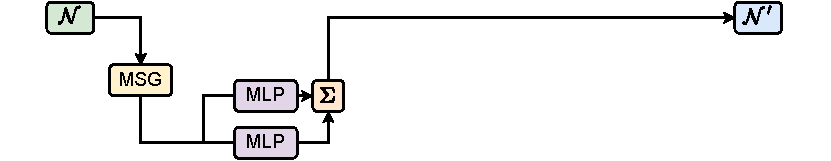
\includegraphics[width=0.99\textwidth]{figures/flavour_tagging/gna.pdf}
    \caption{Diagram of the operations within one graph network layer of the GNA tagger.}
    \label{fig:gna_graph}
\end{figure}

\begin{algorithm}
    \caption{The full GN++ block. All weight calculations are followed by a softmax operation and square brackets denote concatenation.}
    \label{alg:gnpp}
    \begin{algorithmic}[1]
        \State \textbf{Input:} Graph attributes $\mathcal{G} = (\mathcal{N}, \mathcal{E}, \u)$
        \State \textbf{Output:} Updated graph attributes $\mathcal{G}' = (\mathcal{N}', \mathcal{E}', \u')$
        \For{each edge $\edge_k$ in $\mathcal{E}$}
            \State $\edge_k' \gets \text{MLP}_e(\lnorm[\edge_k, \x_{s_k}, \x_{r_k}, \u]) + \edge_k$ \Comment{residual update to edge features}
            \State $\w_k \gets \text{MLP}_{e \to x}(\lnorm[\edge_k, \x_{s_k}, \x_{r_k}, \u])$ \Comment{calculate edge weights}
        \EndFor
        \For{each node $\x_i$ in $\mathcal{N}$}
            \State $\mathbf{\bar\edge}_i \gets \sum_{k: r_k = i} \w_k \edge_k'$ \Comment{attention pool edges}
            \State $\x_i' \gets \text{MLP}_v(\lnorm[\mathbf{\bar\edge}_i, \x_i, \u]) + \x_i$ \Comment{residual update to node features}
            \State $\w_i \gets \text{MLP}_{x \to u}(\lnorm[\mathbf{\bar\edge}_i, \x_i, \u])$ \Comment{calculate node weights}
        \EndFor
        \State $\mathbf{\bar{x}} \gets \sum_{i} \w_i \x_i'$ \Comment{attention pool nodes}
        \State $\u' \gets \text{MLP}_u(\lnorm[\mathbf{\bar{x}}, \u]) + \u_i$ \Comment{residual update to global attributes}
    \end{algorithmic}
\end{algorithm}

\subsection{Spice}

The Spice model is based on the transformer-encoder architecture described in \Cref{sec:transformer} with PreNorm and LayerScale.
A diagram showing the information flow similarly as the other models is shown in \Cref{fig:spice_graph}.
The model is composed of TE Blocks, each with 4 attention heads.
For the nodewise updates we use the same MLPs as GN++.
For constructing a pooled graph representation we use three CA Blocks, also with 4 attention heads, to aggregate the embedded tracks into a single learnable class token.
This pooled representation is then used similarly to GN1 in three separate MLPs for the graph, node, and edge tasks.
The main hyperparameters of the model is the embedding dimension and the number of TE Blocks, which we allow to vary to investigate the scaling capabilities of the tagger.
The model was implemented using standard PyTorch operations.

\begin{figure}[h!]
    \centering
    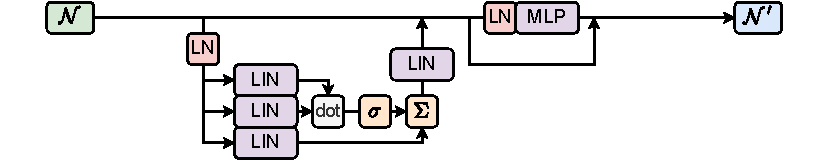
\includegraphics[width=0.99\textwidth]{figures/flavour_tagging/spice.pdf}
    \caption{Diagram of the operations within one transformer layer of the Spice tagger.}
    \label{fig:spice_graph}
\end{figure}

\section{Training}

We reuse the same training loss as GN1, which involves weighted sum of three loss terms,
\begin{equation}
    \mathcal{L} = \mathcal{L}_{\text{graph}} + \alpha \mathcal{L}_{\text{node}} + \beta \mathcal{L}_{\text{edge}},
\end{equation}
The graph loss $\mathcal{L}_{\text{graph}}$ is a cross-entropy loss between the predicted jet flavour and the ground truth.
No balancing is required due to the resampling of the training set.
The node loss $\mathcal{L}_{\text{node}}$ is calculated similarly but for the track origin task and averaged over all tracks in the batch.
The cross entropy calculation for this task is weighted by the inverse frequency of each type of label in \Cref{tab:track_labels} across the training set to account for class imbalance.
The edge loss $\mathcal{L}_{\text{edge}}$ is calculated using a binary cross entropy between the predicted vertex label and the ground truth.
The weight for each pair of tracks is set to 2 if the tracks pair is from a $b$- or $c$-hadron decay, and 1 otherwise.
This enforces the model to focus on heavy flavour vertices.
The total loss is averaged over all jets in the batch.
This does imply that jets with more tracks have a larger contribution to the loss, due to more terms in the track and track pairs, but we found this effect to be minimal.

We keep the same loss coefficients as GN1, $\alpha = 0.5$ and $\beta = 1.5$.
We ran ablation studies to determine the effect of the different tasks on the overall performance of the model, and these are included in the results.

The main training configuration was as follows.
The batch size was set to 1024 and the learning rate followed a cyclic schedule with a period of 5 epochs.
The minimum learning rate was set to $1.0 \times 10^{-5}$ and the maximum to $5.0 \times 10^{-4}$.
We found that the warm-up period was necessary to prevent the model from diverging.
We used the AdamW~\cite{AdamW} optimizer with a weight decay of $1.0 \times 10^{-4}$.
Training was performed for 50 epochs and the checkpoint with the lowest validation loss was saved for evaluation.
Gradient clipping was applied with a maximum norm of 10.
For the graph network grid search, we limited training to only 5 epochs, matching one cycle of the learning rate schedule.

\section{Results}

The performance of all models is evaluated separately using the two test datasets.
For these comparisons we also individually evaluate the $b$-tagging and $c$-tagging performance.
To turn the three class output into a single $b$-tagging score we use the following formula,
\begin{equation}
    D_b = \log\frac{p_b}{(1-f_c)p_l + f_c p_c},
\end{equation}
where $p_b$, $p_c$, and $p_l$ are the probabilities of the jet being a $b$-, $c$-, and light-jet respectively, and $f_c$ is a free parameter that provides a trade-off between $c$- and light-jet rejection.
The choice of $f_c$ is arbitrary and in GN1 it is set to $0.05$, but for our models we found a better balance at $0.02$.
This procedure may also be used to construct a $c$-tagging score $D_c$ with an equivalent $f_b$ parameter.
We set $f_b = 0.2$ for the $c$-tagging scores, matching the GN1.

The performance of tagging algorithms is typically quantified by the rejection rate $r_B$ for various backgrounds at signal efficiency $\epsilon_S$ working points (WP).
The background rejection is defined as the reciprocal of the background efficiency $r_B = \sfrac{1}{\epsilon_B}$.
The standard efficiency WP $b$-tagging algorithms in ATLAS are 60\%, 70\%, 77\%, and 85\%, while the WPs for $c$-tagging are considerably lower, with a WP of 25\% being a common choice.
Thus to better compare the models, we use receiver operating characteristic (ROC) curves, allowing us to measure the performance of the model at all possible operating points.

\subsection{Graph Ablation Studies}

In order to test if each of the proposed changes to the graph network to move from GN1 to GN++ are beneficial we perform a grid search over each of the features in \Cref{tab:gnpp_grid}.
The two extremes are the minimal model, GNA which has all of these features deactivated and the maximal model and is close to GN1, and the maximal model GN++, which has all of these features activated.
For this section only we limit the training to 5 epochs to reduce the computational cost.

To capture overall trends on the inclusion of these features we can use the $\mathcal{L}_{\text{graph}}$ as measured on the test set.
This is shown in the violin plots of \Cref{fig:violin} which can capture first order effects.
This indicates that the most important feature is the use of persistent edge information, followed by nodewise feed-forward updates.
However, all features are beneficial, and the best performance was achieved by the maximal model GN++.
The least significant feature is the use of PreNorm, which we found to be only beneficial when used in combination with residual connections and node feed-forward updates.

\begin{figure}[ht]
    \centering
    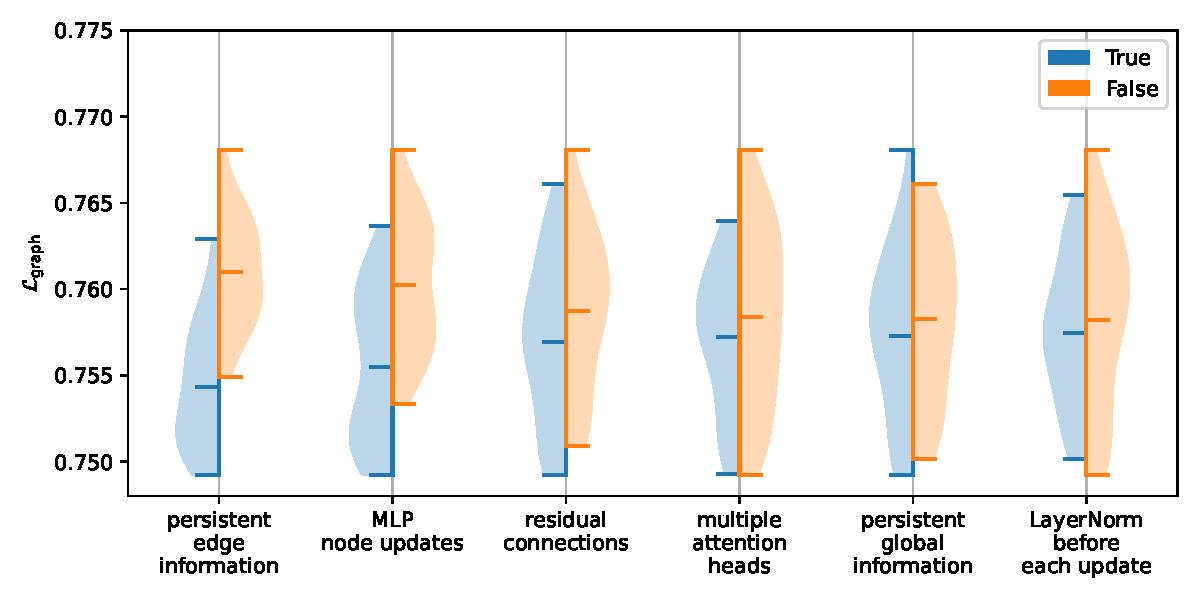
\includegraphics[width=0.99\textwidth]{figures/flavour_tagging/violin.pdf}
    \caption{Violin plots showing the distribution of the graph loss $\mathcal{L}_{\text{graph}}$ for the grid search over the GN++ features grouped by whether the feature is activated.}
    \label{fig:violin}
\end{figure}

We can further investigate this by looking at an ablation study of the performance of the $b$-tagging scores $\ttbar$ sample.
For each feature we compare four models, GNA, GNA with the feature activated, GN++, and GN++ with the feature deactivated.

The results for the two most important features, persistent edge information and nodewise feed-forward updates, are shown in \Cref{fig:ablation}.
For this sample the GN++ tagger is the best performing model, with around 25\% increase in both light and $c$-jet rejection at the 70\% WP.
At the high efficiency WP of 85\% the improvement drops to around 20\% and 15\% for light and $c$-jets respectively.
Interestingly, the persistent edge information seems to be such a crucial feature that activating only this feature results in a more performant tagger than one with all others activated.
The inclusion of only nodewise feed-forward barely improves the performance of the model, but when combined the other features which assist in stabilizing the training, the performance is significantly improved.

\begin{figure}[ht]
    \centering
    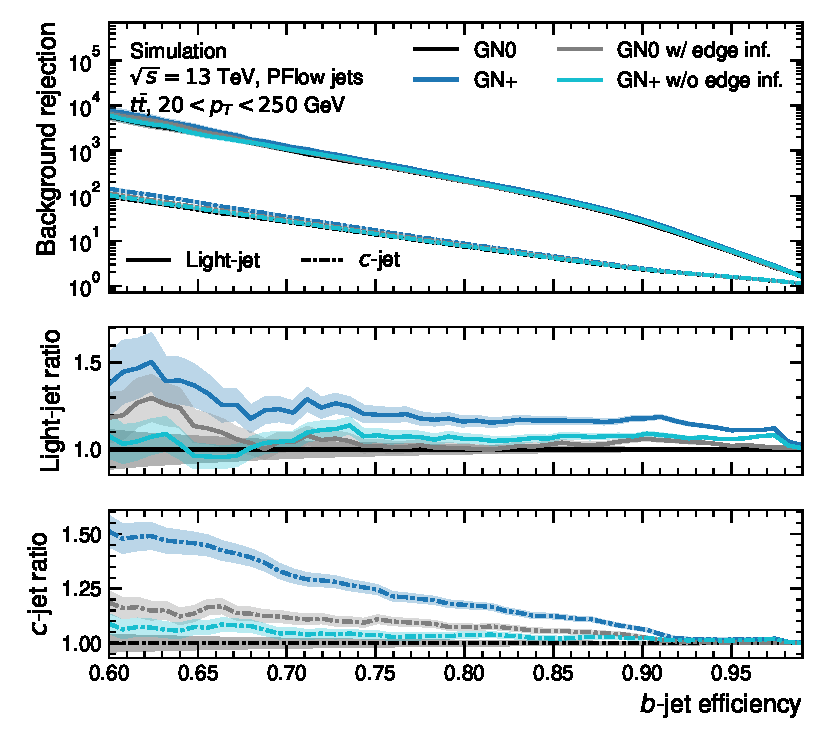
\includegraphics[width=0.49\textwidth]{figures/flavour_tagging/b_roc_ttbar_edge.pdf}
    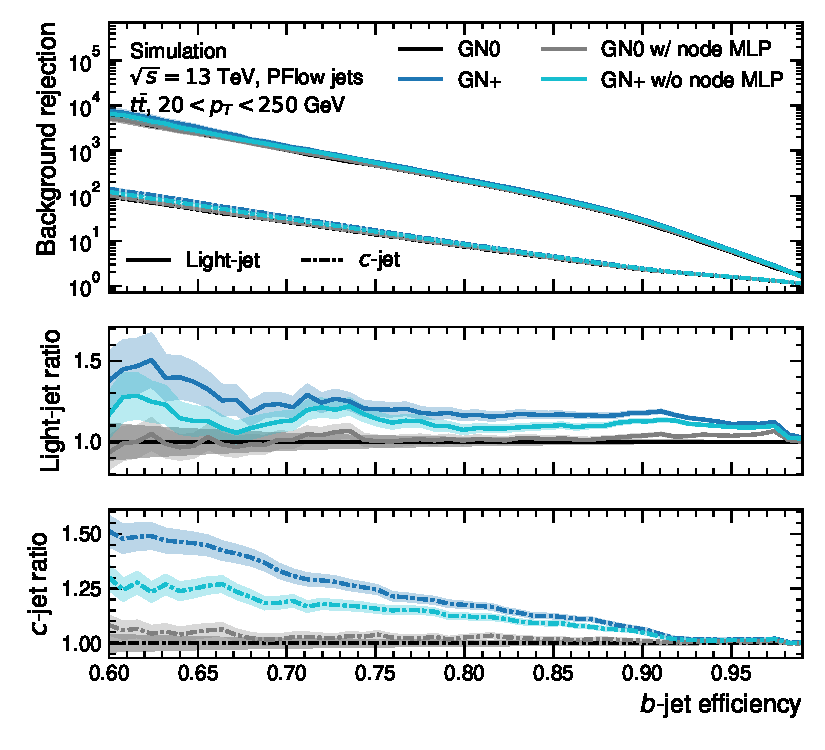
\includegraphics[width=0.49\textwidth]{figures/flavour_tagging/b_roc_ttbar_node.pdf}
    \caption{ROC curves for the $b$-tagging scores for $\ttbar$ jets with $20 < \pt < 250~\GeV$. The rejection values are calculated separately for light- and $c$-jets. The bottom two panels show the ratio of these rejection values to the GNA tagger. The error bands show binomial uncertainties. The left plots show the effect of activating persistent edge information in the graph network and the right plots show the effect of activating nodewise feed-forward updates.}
    \label{fig:ablation}
\end{figure}

\subsection{Tagging Performance vs GN1}

When comparing to GN1, we look at the performance of both $b$- and $c$-tagging scores for the $\ttbar$ and $Z'$ samples.
We use the ROC curves to compare the performance of the models at all possible operating points, but we also show specific values for the 70\% WP for $b$-tagging and the 25\% WP for $c$-tagging in \Cref{tab:roc}.

To ensure a fair comparison, we introduce model of various sizes, with some having roughly the same number of trainable parameters as GN1.
The GN++ model has 780k trainable parameters, while the GN1 model has 820k, thus we design a Spice variant with approximately 800k.
This model has 7 TE Blocks and an embedding dimension of 64.
We then investigate how these models scale by introducing two new transformers, Spice-large and Spice-huge.
Both use the same number of layers, but Spice-large has an embedding dimension of 128 and Spice-huge has an embedding dimension of 256\footnote{Note that the FFN dimensions always double the embedding dimension.}.
These correspond to 1.4M and 4.2M trainable parameters respectively.
We also introduce GN++large which also has an embedding dimension of 128, leading to 1.6M trainable parameters.

The results for the $\ttbar$ sample are shown in \Cref{fig:ttbar_roc}.
For the models with the same number of parameters as GN1, both new models outperform it given a signal jet efficiency of less than 90\%.
For $b$-tagging at the 70\% WP, Spice yields around 50\% improvement in light-jet rejection and around 35\% improvement in $c$-jet rejection with respect to GN1.
The larger models further increase this performance gain, with Spice-huge offering a 70\% improvement in light-jet rejection and 60\% improvement in $c$-jet rejection.
For $c$-tagging, most of the performance improvement is for much lower signal efficiencies.
At the 25\% WP, Spice improves over GN1 by 18\% in $b$-jet rejection and 40\% in light-jet rejection.
It is interesting that Spice is consistently better than GN++ for both $b$- and $c$-tagging on this dataset, as it lacks the feature determined to be the most important in the ablation studies, the persistent edge information.
However, these models are trained for 10 times longer than the ablation studies, so it is possible that the transformer based model is able to learn the same information in a more efficient manner.
Once again, the most performant model is Spice-huge, which is able to achieve a 25\% $b$-jet rejection improvement and 50\% light-jet rejection improvement over GN1 at the 25\% $c$-tagging WP.

The results for the much higher $\pt$ $Z'$ sample are shown in \Cref{fig:zprime_roc}.
All models once again outperform GN1.
For the smaller networks GN++ provides higher rejection rates than Spice.
These jets have an order of magnitude higher $\pt$ than the $\ttbar$ jets, and the GN++ model seems to be better suited for this data type.
However, by scaling the models, Spice-large is easly able to outperform GN++ and even GN++large.
It achieves and improvement of



\begin{figure}[ht]
    \centering
    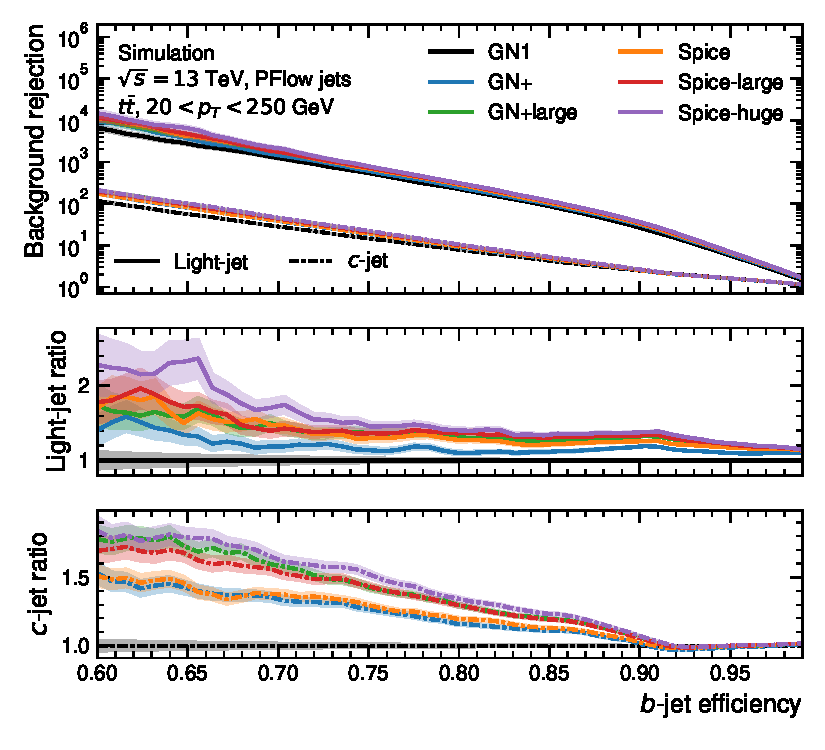
\includegraphics[width=0.49\textwidth]{figures/flavour_tagging/b_roc_ttbar_large.pdf}
    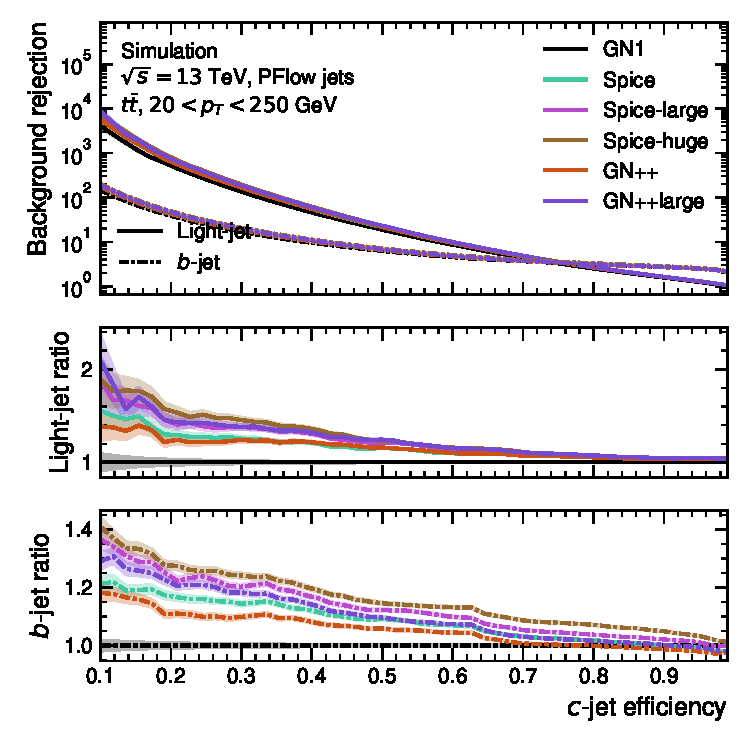
\includegraphics[width=0.49\textwidth]{figures/flavour_tagging/c_roc_ttbar_large.pdf}
    \caption{ROC curves for the $b$-tagging scores (left) and $c$-tagging scores (right) for $\ttbar$ jets with $20 < \pt < 250~\GeV$. The rejection values are calculated separately for each background type. The bottom two panels show the ratio of these rejection values to the GN1 tagger. Error bands are derived from binomial uncertainties.}
    \label{fig:ttbar_roc}
\end{figure}

\begin{figure}[ht]
    \centering
    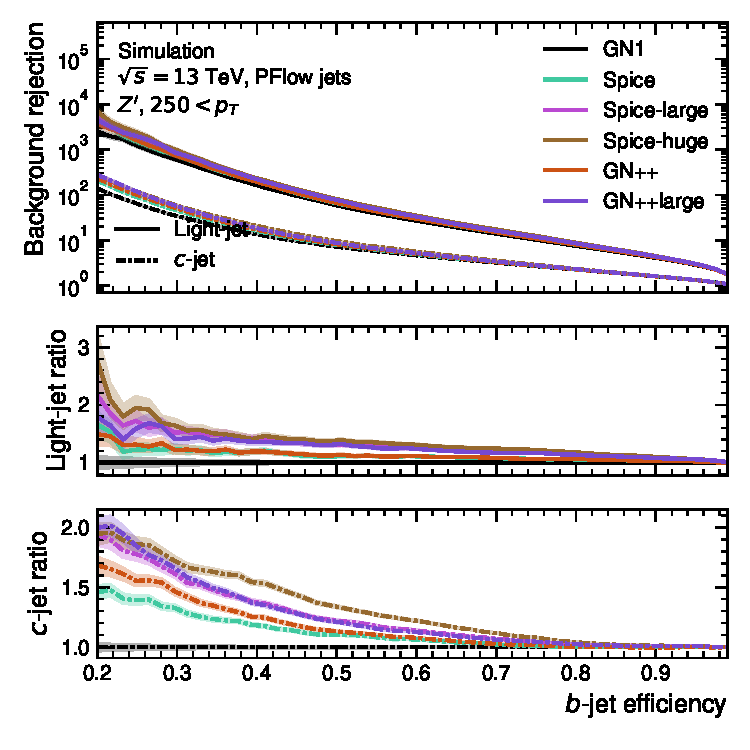
\includegraphics[width=0.49\textwidth]{figures/flavour_tagging/b_roc_zprime_large.pdf}
    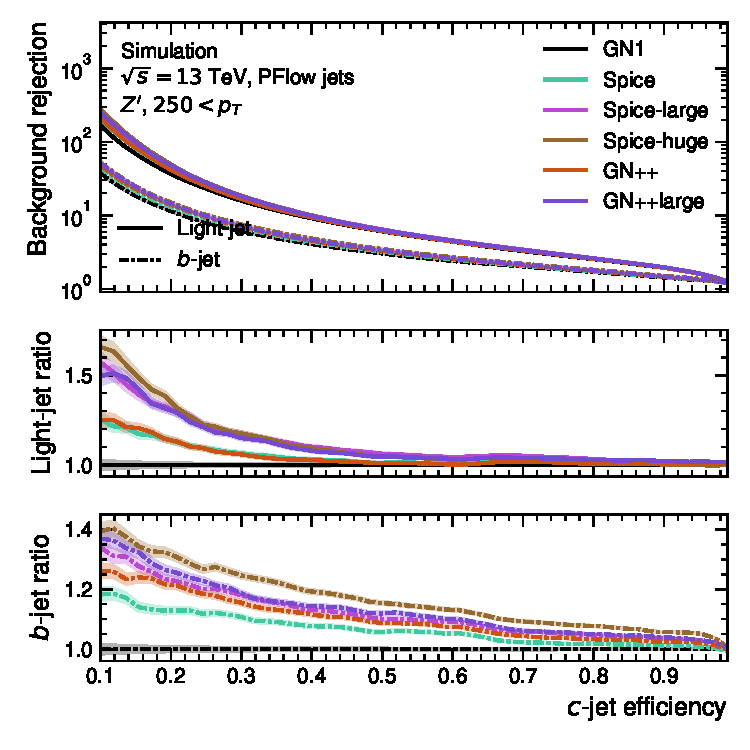
\includegraphics[width=0.49\textwidth]{figures/flavour_tagging/c_roc_zprime_large.pdf}
    \caption{ROC curves for the $b$-tagging scores (left) and $c$-tagging scores (right) for $Z'$ jets with $\pt > 250~\GeV$. The rejection values are calculated separately for each background type. The bottom two panels show the ratio of these rejection values to the GN1 tagger. Error bands are derived from binomial uncertainties.}
    \label{fig:zprime_roc}
\end{figure}

\begin{table}[ht]
    \centering
    \begin{tabular}{l@{\hskip 30pt}cc@{\hskip 20pt}cc@{\hskip 35pt}cc@{\hskip 20pt}cc@{\hskip 20pt}}
        \toprule
        & \multicolumn{4}{c@{\hskip 35pt}}{$\ttbar$} & \multicolumn{4}{c@{\hskip 20pt}}{$Z'$} \\
        & \multicolumn{2}{c@{\hskip 20pt}}{$\epsilon_S^b=75\%$} & \multicolumn{2}{c@{\hskip 35pt}}{$\epsilon_S^c=25\%$}
        & \multicolumn{2}{c@{\hskip 20pt}}{$\epsilon_S^b=75\%$} & \multicolumn{2}{c@{\hskip 20pt}}{$\epsilon_S^c=25\%$} \\
        & $r_B^c$ & $r_B^l$ & $r_B^b$ & $r_B^l$ & $r_B^c$ & $r_B^l$ & $r_B^b$ & $r_B^l$ \\
        \midrule
        Spice & 38 & 47 & 16 & 27 & 2 & 8 & 12 & 9 \\
        Spice-large & 54 & 41 & 23 & 38 & 7 & 21 & 20 & 22 \\
        Spice-huge & \textbf{63} & \textbf{73} & \textbf{26} & \textbf{50} & \textbf{12} & \textbf{25} & \textbf{27} & \textbf{22} \\
        GN++ & 34 & 19 & 10 & 22 & 3 & 8 & 18 & 9 \\
        GN++large & 59 & 46 & 21 & 42 & 6 & 17 & 23 & 21 \\
        \bottomrule
    \end{tabular}
    \caption{Comparison of $b$- and $c$-tagging scores for $\ttbar$ and $Z'$ samples across different models.}
    \label{tab:comparison}
\end{table}

\subsubsection{Computational Cost}

Key to this study is the computational cost of these models.
The GPU and CPU times for inference with respect to all models are shown in \Cref{tab:inference}.
The GN++ models are the slowest to run on both the CPU and GPU.
This is likely due to the inefficient implementation of the graph layers in the custom graph library.
This is in contrast to the transformer based models which barely increase in inference time when running on the GPU as so many of the operations are basic matrix multiplications and thus highly parallelized.
Even though the expressivity of a single GN++ layer is theoretically much higher than a single transformer layer, the efficienty of the latter allows it to outscale the former.


\begin{table}
    \centering
    \begin{tabular}{lrrr}
        \toprule
        Model & Parameters & GPU Time (ms) & CPU Time (ms) \\
        \midrule
        GN1 & 820k & 0.06 & 1.4 \\
        GN++ & 780k & 0.50 & 23.0 \\
        GN++large & 1.6M & 0.90 & 59.0 \\
        Spice & 800k & 0.03 & 1.5 \\
        Spice-large & 1.4M & 0.05 & 4.4 \\
        Spice-huge & 4.2M & 0.08 & 7.3 \\
        \bottomrule
    \end{tabular}
    \caption{Inference times for the different models on a CPU (AMD EPYC 7742) and GPU (NVIDIA 3090).}
    \label{tab:inference}
\end{table}

The performance of the larger models are shown in \Cref{fig:ttbar_large} and \Cref{fig:zprime_large}.


\section{GN2 Tagger}

% - Salt
% - GN2X
% - Current model architecture
% - Current training set
% - Current performance
% - Future work
% GN3 and and neutrals
% Put in that we want to do smarter vertexing, maybe with attention maps





